\subsubsection{Kommunikationsmodul}
\begin{figure}[h]
\centering
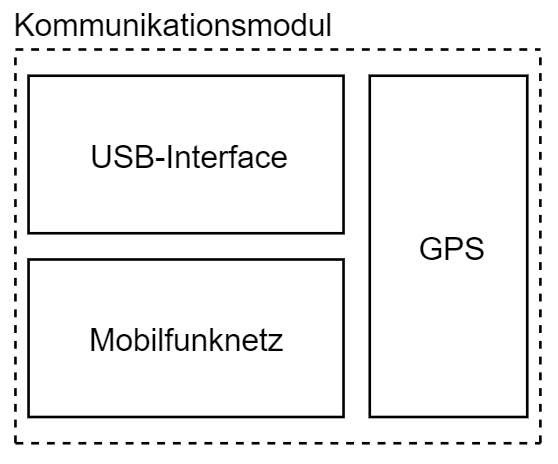
\includegraphics[scale=0.7]{graphics/Konzeptdiagramme/Kommunikationsmodul.PNG}
\caption{Kommunikationsmodul}
\label{fig:kommunikationsmodul}
\end{figure}
Abbildung \ref{fig:kommunikationsmodul} zeigt die verschiedenen Schnittstellen, über welche Daten mit der Umgebung (User) und \textit{MCU} ausgetauscht werden können. Im Rahmen eines vorhergehenden Projekts wurde das USB-Interface umgesetzt. Mobilfunknetz und GPS sind Teil von diesem Projekt.\\

\subparagraph{USB-Interface:}
Über dieses Interface kann mit dem System kommuniziert und interagiert werden. Ein serielles Terminal-Emulationsprogramm (wie z.B. PuTTY) wird dazu benötigt.\\

\subparagraph{Mobilfunknetz:}
Die mobile Wetterstation soll mittels SMS abgefragt werden können. Um dies zu bewerkstelligen, wird ein GSM-Modul benötigt, welches auf dem PCB integriert werden kann. Ein GSM-Modul benötigt eine SIM-Karte, welche zur Identifikation des Nutzers dient. Das Modul empfangt digitale Befehle via SMS und leitet diese über eine serielle Schnittstelle weiter zur eigenen MCU, worin diese Befehle verarbeitet werden und eine Antwort-SMS auslösen. Die Form der Antwort-SMS soll erst im weiteren Verlauf des Projekts festgelegt werden. Ferner wäre es von Vorteil die erhobenen Daten auf einen Server zu Uploaden, damit Daten für die Klimaforschung gesammelt werden können, was jedoch als Wunschziel definiert wurde. Es ist ebenso möglich die mobile Wetterstation in das \textit{IoT} (Internet of Things) zu implementieren, womit die Datenerfassung der Sensorik sich in Echtzeit verfolgen lässt, was jedoch ebenso ein Wunschziel des Projekts ist. \\

\subparagraph{GPS:}
Um den Standort der mobilen Wetterstation zu ermitteln, wird ein GPS-Modul implementiert. Ein GPS-Modul errechnet die Laufzeiten der Signale der Satelliten bis zum Empfänger. Dadurch, dass die Ausbreitungsgeschwindigkeit von elektromagnetischen Wellen bekannt ist (Lichtgeschwindigkeit), kann auf die Entfernung zurückgerechnet werden. Mittels Triangulation (wenn die Entfernung zu 3 Satelliten bekannt ist) erfolgt schliesslich die Positionsbestimmung. Dazu muss das GPS-Modul über die Positionsdaten der Satelliten verfügen, die mit Hilfe bestimmter Daten errechnet werden, welche als Datensatz dem Empfängermodul vorliegen. Die Positionsbestimmung ist jedoch ebenso abhängig von Umgebungsfaktoren wie z.B. Berge oder hohe Gebäude, weshalb in diesem Projekt keine exakte Positionsbestimmung garantiert werden kann.\\